\documentclass[a4paper,11pt]{article}
\usepackage[utf8]{inputenc}
\usepackage[german]{babel}
\usepackage{geometry}
\usepackage{graphicx}
\usepackage{float}
\usepackage{parskip}
\usepackage{titlesec}
\usepackage{hyperref}

\setcounter{secnumdepth}{4}

\titleformat{\paragraph}
{\normalfont\normalsize\bfseries}{\theparagraph}{1em}{}
\titlespacing*{\paragraph}
{0pt}{3.25ex plus 1ex minus .2ex}{1.5ex plus .2ex}

\geometry{a4paper, margin=2.5cm}
\graphicspath{{images/}}

\begin{document}

\begin{table}[h]
	\centering
	\footnotesize
	\begin{tabular}{| p{1.5cm} | p{2.5cm} | p{2cm} | p{2cm} | p{2cm} |}
		\hline
		                            & Verantwortliche Teammitglieder (Organisation, Anlegen der Dokumentenversion, Moderation, Abgabe)         & Anwesende während der Meetings                                                                           & (Online-) Beiträge zum Inhalt durch                                                                      & Korrektur-gelesen durch                                                                                  \\
		\hline
		Dokument Sprint 4 Version 1 & Paul Schröder, Eric Buthmann, Yanik Buthmann, Mathis Behrendt, Adrian Gode, Niklas Krüger, Kevin Zellmer & Paul Schröder, Eric Buthmann, Yanik Buthmann, Mathis Behrendt, Adrian Gode, Niklas Krüger, Kevin Zellmer & Paul Schröder, Eric Buthmann, Yanik Buthmann, Mathis Behrendt, Adrian Gode, Niklas Krüger, Kevin Zellmer & Paul Schröder, Eric Buthmann, Yanik Buthmann, Mathis Behrendt, Adrian Gode, Niklas Krüger, Kevin Zellmer \\
		\hline
	\end{tabular}
\end{table}

\section{Backlogs und Planung}

\subsection{Produktbacklog vor und nach dem Sprint}
In diesem Sprint wurden dem Produktbacklog mehrere Tasks hinzugefügt.
Die Tasks wurden in einem Meeting mit den Entwicklern identifiziert.
In diesem Meeting wurde die gesamte Anwendung nach Problemen und Verbesserungsmöglichkeiten durchsucht.
Folgende Tasks sind dadurch entstanden:
\begin{itemize}
	\item Refactoring der Startseite
	\item Refactoring des Headers
	\item Refactoring User Story S5.3: Anzeige Profil
	\item Refactoring für User Story S2.2: Bug-Fix Priorität einer User Story wird beim Speichern nicht übernommen
	\item Refactoring für User Story S3.3: Anzeige und Sortierung von Task-Prioritäten im Backlog
	\item Refactoring Anzeige Assignees
	\item Vereinheitlichung der Sprache
	\item überflüssige Zurück-Buttons entfernen
	\item Umleitung nach Registrierung korrigieren
	\item Fehler in Suche beheben
\end{itemize}

\subsection{Sprint Planung}
Im letzten Sprint wurden alle verbleibenden User Stories und Anforderungen vollständig umgesetzt.\\
In diesem Sprint lag der Fokus auf Refactoring sowie der Erweiterung und Korrektur bereits implementierter Features.
Die Aufgaben, welche dem Produktbacklog hinzugefügt wurden, sollen in diesem vollständig abgearbeitet werden.\\
\\
\noindent\textit{Hinweis: Das vollständige Sprintbacklog ist unter \href{run:./Sprintbacklog.pdf}{Sprintbacklog.pdf}, sowie \href{https://git.informatik.uni-rostock.de/softwaretechnik-ws-2025-26/uebung3/team3/projekt-team3-uebung3/-/blob/main/abgabedokumente/Sprintbacklog.pdf?ref_type=heads}{im Gitlab} zu finden.}

\section{Verfeinerte Architektur}
\subsection{Task/User Stories}


\subsubsection{Modellierung/Refactoring für User Story S3.3: Anzeige und Sortierung von Task-Prioritäten im Backlog}
\paragraph{Modellierung verfeinerter Struktur}
Die grundlegende Architektur aus Sprint 3 bleibt unverändert. Im Data Layer wurde die Klasse \texttt{Task} um die Hilfsmethode \texttt{getPriorityColor()} ergänzt, die je nach Prioritätswert eine Farbe zurückgibt (rot für Hoch, orange für Mittel, grün für Niedrig). Im Presentation Layer wurde der \texttt{BacklogController} angepasst, sodass die Task-Listen aller fünf Statusspalten vor der Übergabe ans Template nach Priorität absteigend sortiert werden. Im Frontend-Template \texttt{backlog.mustache} wurde jede Task-Karte um ein farbiges Priorität-Badge erweitert.

\paragraph{Modellierung verfeinerter Interfaces und Datenstrukturen}
Es wurden keine neuen Klassen, Interfaces oder Datenbankfelder hinzugefügt. Die bestehende Methode \texttt{getPriorityCount()} aus Sprint 3 wurde lediglich durch \texttt{getPriorityColor()} für die Darstellung ergänzt. Das Klassendiagramm und die Datenstrukturen aus Sprint 3 sind weiterhin gültig.

\paragraph{Modellierung relevanter Verhaltensaspekte}
Beim Aufruf von \texttt{GET /backlog/\{id\}} werden die Tasks wie bisher nach Status gruppiert und nun zusätzlich innerhalb jeder Gruppe nach Priorität absteigend sortiert. Das Sequenzdiagramm aus Sprint 3 beschreibt den Ablauf weiterhin korrekt; Sortierung und Badge-Darstellung sind rein technische Ergänzungen ohne neue Interaktionsschritte.

\subsubsection{Modellierung/Refactoring für User Story S2.2: Bug-Fix Priorität einer User Story wird beim Speichern nicht übernommen}
\paragraph{Modellierung verfeinerter Struktur}
Die Architektur bleibt unverändert. Der Fehler lag in einem inkonsistenten Formularnamen: Das Template \texttt{edit-user-story.mustache} sendete den Prioritätswert unter dem Feldnamen \texttt{priority}, während \texttt{postEditUserStory} im \texttt{UserStoryController} ihn unter \texttt{priorities} abfragte. Dadurch war \texttt{priorityString} stets \texttt{null} und die Priorität wurde nie gespeichert.

\paragraph{Modellierung verfeinerter Interfaces und Datenstrukturen}
Keine Änderungen an Interfaces oder Datenstrukturen.

\paragraph{Modellierung relevanter Verhaltensaspekte}
Nach der Korrektur liest \texttt{postEditUserStory} den Parameter korrekt unter \texttt{priority}. Das Verhalten entspricht nun dem in Sprint 3 beschriebenen Sequenzdiagramm für S2.2.

\subsubsection{Refactoring Startseite}
Das Refactoring der Startseite hatte keine Auswirkungen auf die Struktur des Systems.
Es wurde ausschließlich die grafische Oberfläche verändert.\\
Vor dem Refactoring wurde auf der Startseite eine Liste der Nutzer, eine Liste der Tasks, eine Suchzeile und Buttons zum Erstellen verschiedener Elemente angezeigt.
Die Startseite vor dem Refactoring ist in Abbildung \ref{fig:startseite_vor_refactoring} zu sehen.
\begin{figure}
	\centering
	\fbox{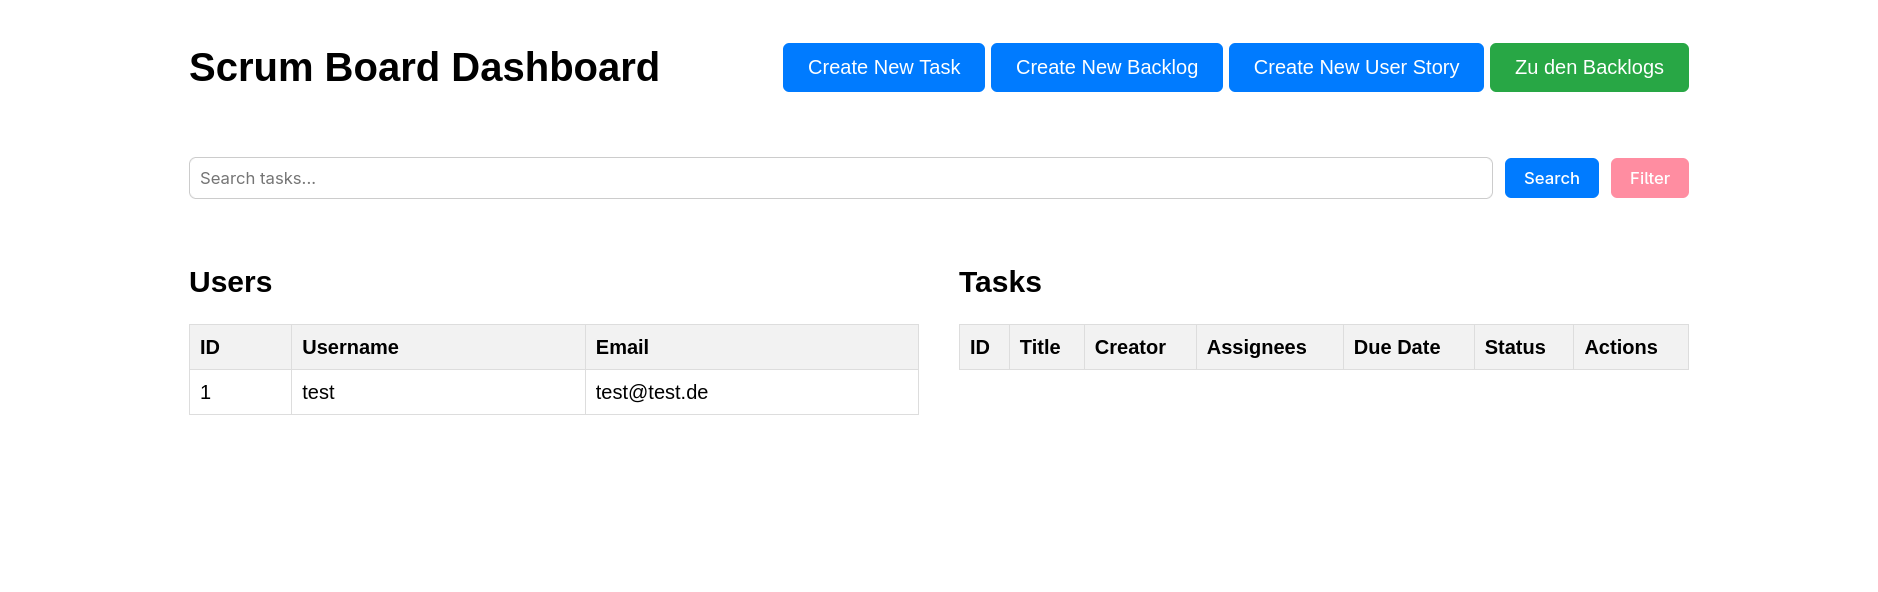
\includegraphics[width=12cm]{startseite_vor_refactoring.png}}
	\caption{Design der Startseite vor dem Refactoring}
	\label{fig:startseite_vor_refactoring}
\end{figure}
Die Entwickler haben sich dazu entschieden, das Hauptfeature, die Backlogs, auf der Startseite anzuzeigen.
Dies soll die Nutzung des Systems vereinfachen.
Die Gestaltung der Startseite nach dem Refactoring ist in Abbildung \ref{fig:startseite_nach_refactoring} zu sehen.
\begin{figure}
	\centering
	\fbox{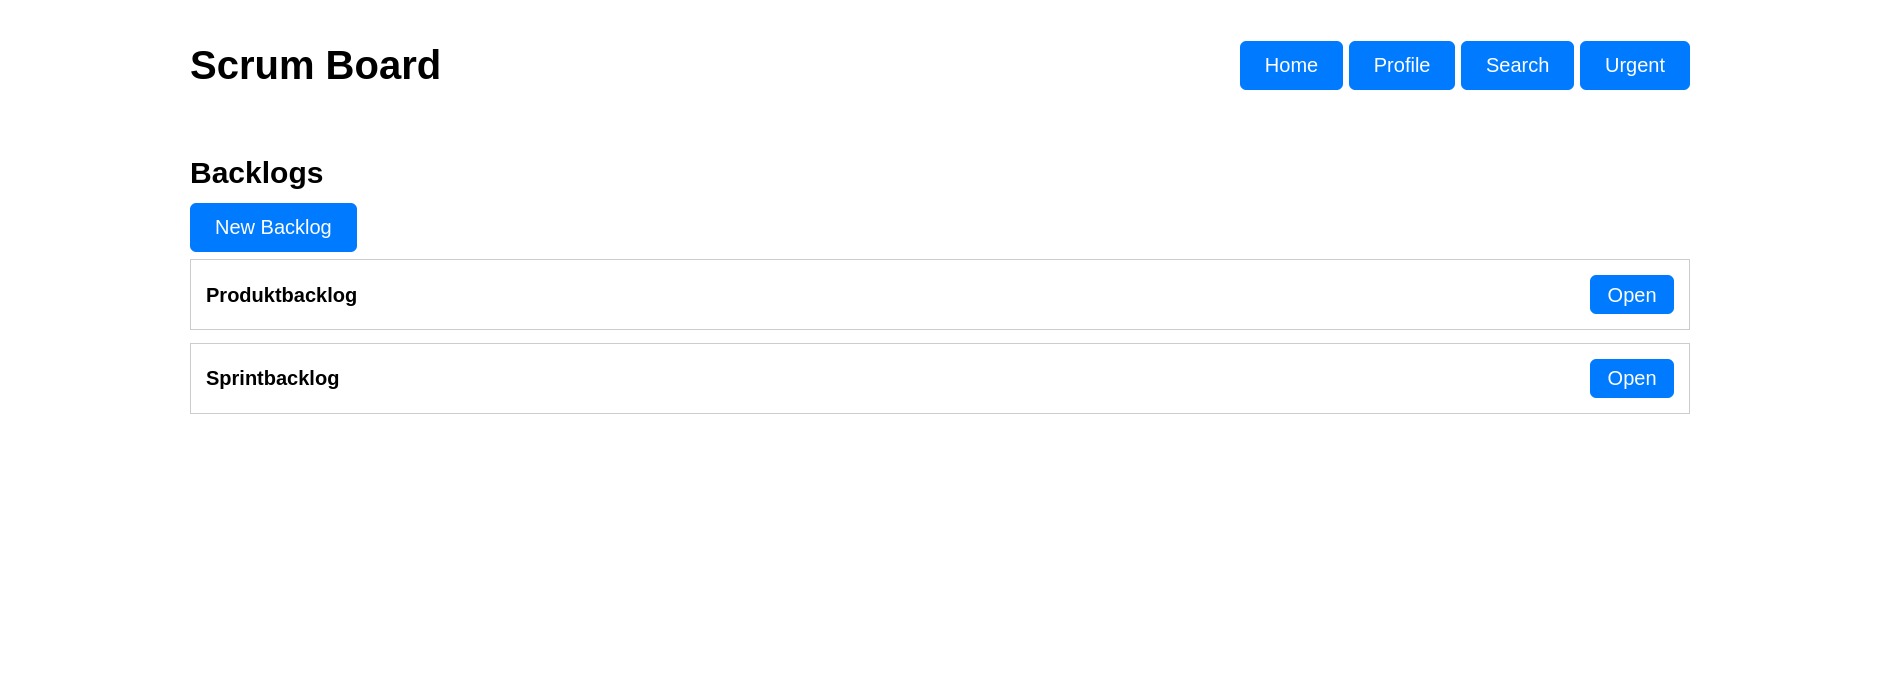
\includegraphics[width=12cm]{startseite_nach_refactoring.png}}
	\caption{Design der Startseite nach dem Refactoring}
	\label{fig:startseite_nach_refactoring}
\end{figure}

\subsubsection{Refactoring Header}
Das Refactoring des Headers hatte keine Auswirkungen auf die Struktur des Systems.
Es wurde ausschließlich die grafische Oberfläche verändert.\\
Das Refactoring des Headers sollte die Anzeige von unterschiedlichen Headern auf den Seiten beheben.
Die Abbildung \ref{fig:header_vor_refactoring} zeigt ein Beispiel für die Anzeige verschiedener Header auf unterschiedlichen Seiten.
\begin{figure}
	\centering
	\begin{minipage}[b]{0.4\textwidth}
		\fbox{
\includegraphics[width=\textwidth]{header_vor_refactoring_1.png}}
	\end{minipage}
	\hfill
	\begin{minipage}[b]{0.4\textwidth}
		\fbox{
\includegraphics[width=\textwidth]{header_vor_refactoring_2.png}}
	\end{minipage}
	\caption{Anzeige unterschiedlicher Header vor dem Refactoring}
	\label{fig:header_vor_refactoring}
\end{figure}
Um dieses Problem zu beheben, wurde ein Mustache-Partial erstellt.
Das Partial wurde dann auf jeder Seite eingebunden.
Damit erhält man auf jeder Seite einen einheitlichen Header.\\
Der einheitliche Header ist in Abbildung \ref{fig:header_nach_refactoring} zu sehen.
\begin{figure}
	\centering
	\fbox{
\includegraphics[width=10cm]{header_nach_refactoring.png}}
	\caption{Einheitlicher Header nach dem Refactoring}
	\label{fig:header_nach_refactoring}
\end{figure}

\subsubsection{Refactoring User Story S5.3: Anzeige Profil}
Das Refactoring der Profilseite hatte keine Auswirkungen auf die Struktur des Systems.
Es wurde ausschließlich die grafische Oberfläche verändert.\\
Die grafische Oberfläche der Profilseite unterschied sich vor dem Refactoring deutlich vom Designkonzept der anderen Seiten.
Zu sehen ist die Oberfläche der Profilseite vor dem Refactoring in Abbildung \ref{fig:profilseite_vor_refactoring}.
\begin{figure}
	\centering
	\fbox{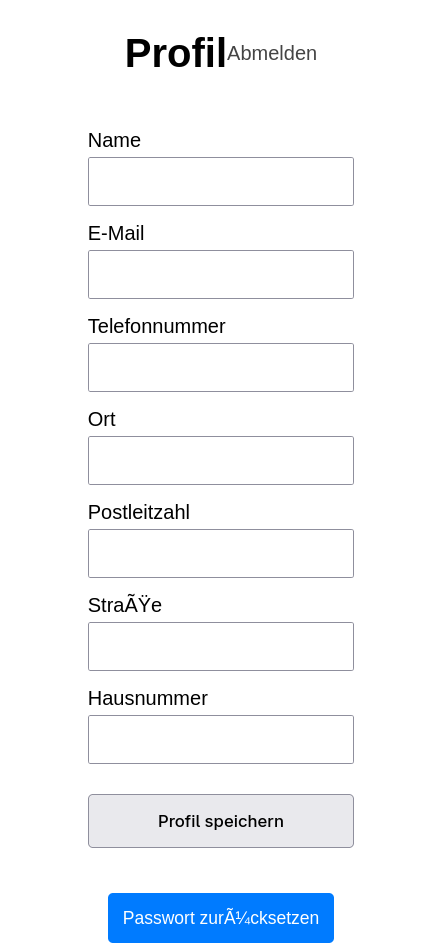
\includegraphics[width=4cm]{profilseite_vor_refactoring.png}}
	\caption{Design der Profilseite vor dem Refactoring}
	\label{fig:profilseite_vor_refactoring}
\end{figure}
Durch das Refactoring wurde die Seite an das allgemeine Designkonzept der Anwendung angepasst.
Zu sehen ist die verbesserte Oberfläche in Abbildung \ref{fig:profilseite_nach_refactoring}.
\begin{figure}
	\centering
	\fbox{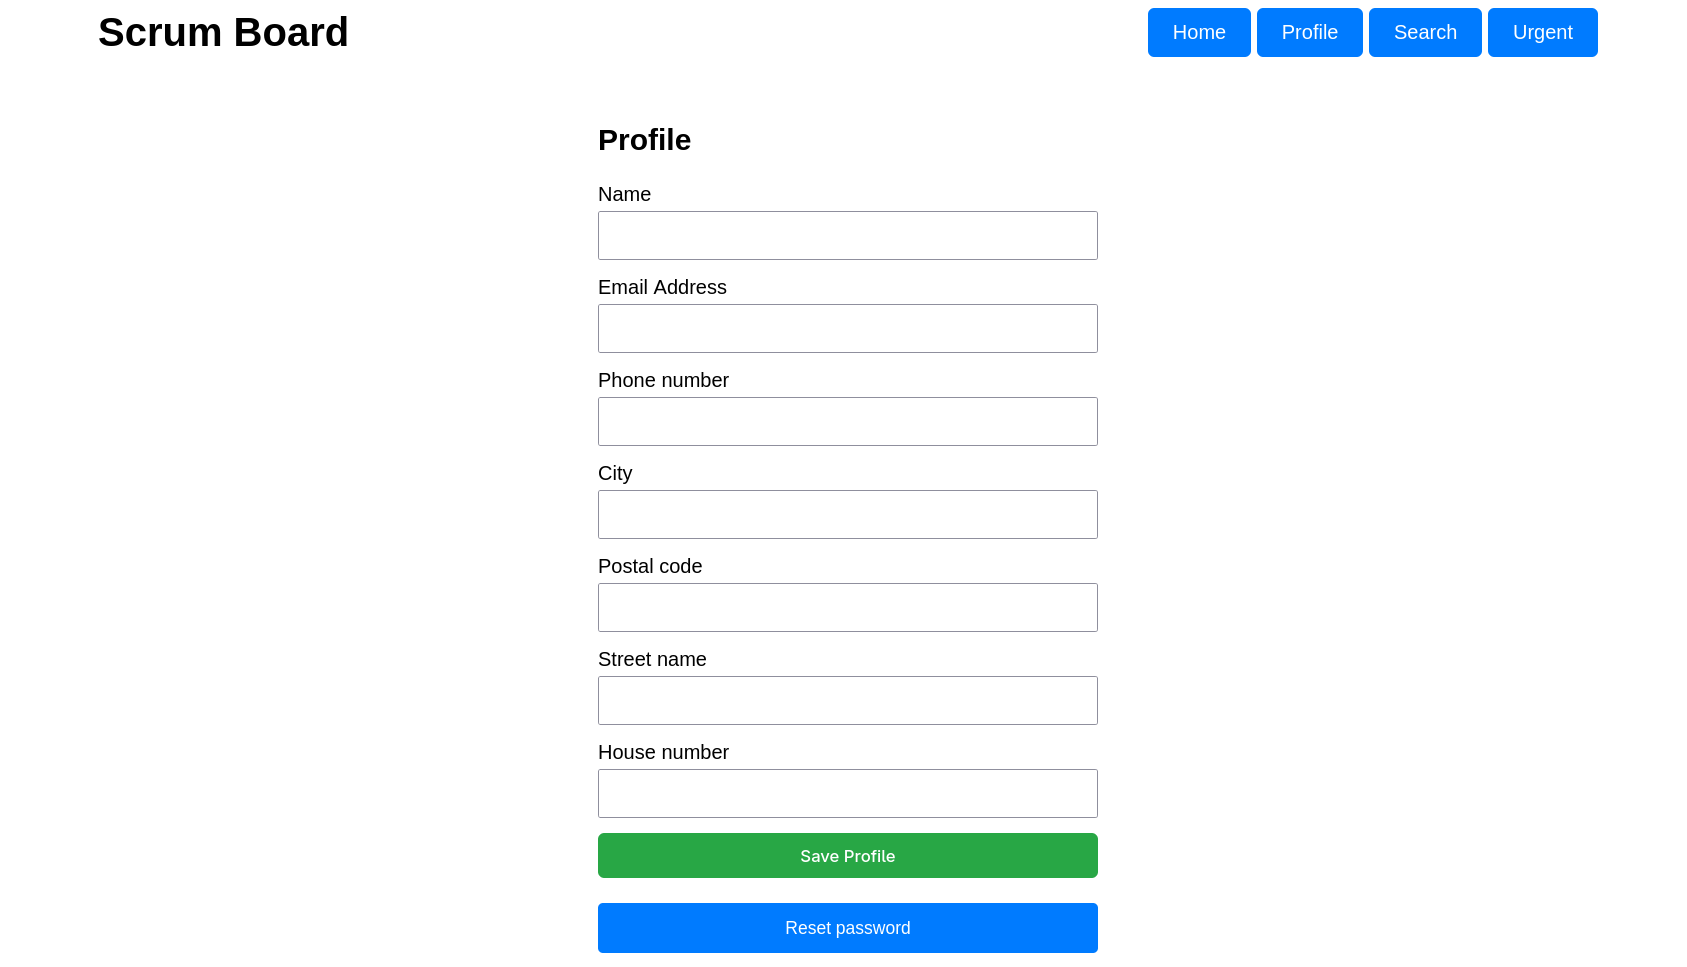
\includegraphics[width=12cm]{profilseite_nach_refactoring.png}}
	\caption{Design der Profilseite nach dem Refactoring}
	\label{fig:profilseite_nach_refactoring}
\end{figure}


\section{Implementation und Tests}
\subsection{Updates zu den genutzten Technologien}
An den genutzten Technologien wurden keine Änderungen vorgenommen.

\subsection{Dokumentation der Codequalität}
Wie in den vorangegangenen Sprints wurde die Korrektheit der Implementierung manuell überprüft.
Für die in diesem Sprint durchgeführten Erweiterungen und Bug-Fixes wurden neue Testfälle erstellt.
Die vollständige Testdokumentation ist im \href{https://git.informatik.uni-rostock.de/softwaretechnik-ws-2025-26/uebung3/team3/projekt-team3-uebung3/-/blob/main/abgabedokumente/Manuelle_Tests.pdf?ref_type=heads}{Gitlab} zu finden.

\subsection{Tracing}
Da der Umfang der Aufgaben stark variierte, wurden einige Aufgaben auf einem separaten Branch und andere wiederum als einzelner Commit auf dem main-Branch umgesetzt.
In Tabelle \ref{tab:tracing} wird daher der Hash des Commits aufgeführt, der alle Änderungen für die jeweilige Aufgabe enthält.
Im Fall von umfangreicheren Aufgaben, ist dies der Merge-Commit.

\begin{table}[H]
	\centering
	\small
	\renewcommand{\arraystretch}{1.4}
	\begin{tabular}{| p{4.5cm} | p{9cm} |}
		\hline
		\textbf{Aufgabe}                                          & \textbf{Hash des Commits}                \\
		\hline
		Refactoring Startseite                                    & e11f1598abe405648113fe816094e33a38ac638e \\
		\hline
		Refactoring Profilseite                                   & 21fb79bf713f3093c29d9445bdc81d7e376d493a \\
		\hline
		Refactoring Header                                        & 0d590a2623358612f4ce1229d06cee310e629163 \\
		\hline
		\textbf{S3.3} - Priorität-Badge und Sortierung im Backlog & 7e139701164b596093647577f7a605dff54a0921 \\
		\hline
	\end{tabular}
	\caption{Tracing: Hashes der Commits}
	\label{tab:tracing}
\end{table}

\subsection{Laufender Prototyp}
Der aktuelle Prototyp erfüllt alle im Dokument \href{https://git.informatik.uni-rostock.de/softwaretechnik-ws-2025-26/uebung3/team3/projekt-team3-uebung3/-/blob/main/anforderungen/anforderungen.pdf?ref_type=heads}{Anforderungen} genannten Anforderungen.

\subsubsection*{Installations- und Kompilieranweisung}
Die Installations- und Kompilieranweisung ist im \href{https://git.informatik.uni-rostock.de/softwaretechnik-ws-2025-26/uebung3/team3/projekt-team3-uebung3/-/blob/main/README.md?ref_type=heads}{Gitlab} zu finden.

\subsection{Abweichung Sprintplanung}
Der Plan in diesem Sprint war es, Refactoring-Maßnahmen durchzuführen sowie bereits implementierte Features zu erweitern und zu korrigieren. Alle geplanten Aufgaben wurden vollständig umgesetzt, sodass der Plan erfüllt wurde.

\end{document}
